% This file was created by matlab2tikz.
%
%The latest updates can be retrieved from
%  http://www.mathworks.com/matlabcentral/fileexchange/22022-matlab2tikz-matlab2tikz
%where you can also make suggestions and rate matlab2tikz.
%
\definecolor{mycolor1}{rgb}{0.00000,0.44700,0.74100}%
\definecolor{mycolor2}{rgb}{0.85000,0.32500,0.09800}%
%
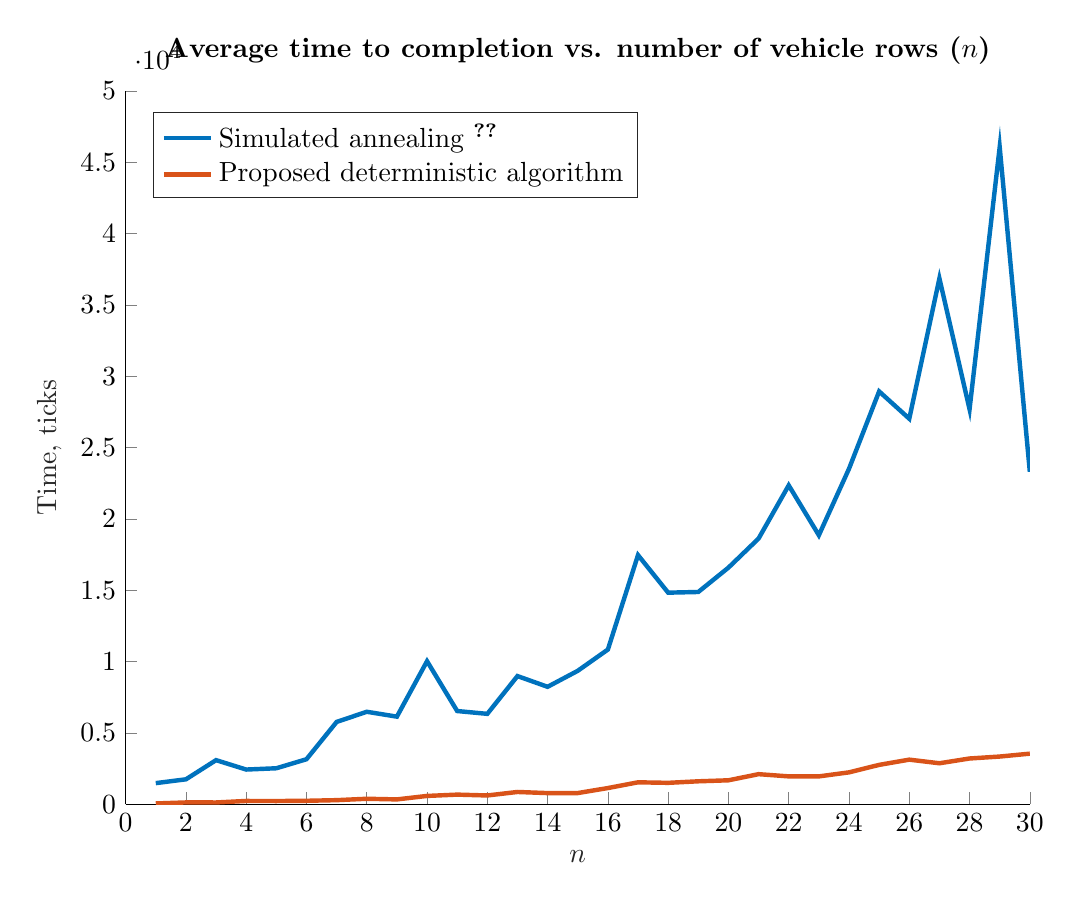
\begin{tikzpicture}

\begin{axis}[%
width=4.521in,
height=3.566in,
at={(0.758in,0.481in)},
scale only axis,
xmin=0,
xmax=30,
xlabel style={font=\color{white!15!black}},
xlabel={$n$},
ymin=0,
ymax=50000,
ylabel style={font=\color{white!15!black}},
ylabel={Time, ticks},
axis background/.style={fill=white},
title style={font=\bfseries},
title={Average time to completion vs. number of vehicle rows ($n$)},
axis x line*=bottom,
axis y line*=left,
every axis plot/.append style={ultra thick},
legend style={at={(0.03,0.97)}, anchor=north west, legend cell align=left, align=left, draw=white!15!black}
]
\addplot [color=mycolor1]
  table[row sep=crcr]{%
1	1474.1975\\
2	1740.8125\\
3	3085.54475703325\\
4	2425.50125313283\\
5	2516.0925\\
6	3149.14070351759\\
7	5762.06811989101\\
8	6476.55524861879\\
9	6134.5790960452\\
10	10022.1516245487\\
11	6527.96875\\
12	6330.07304785894\\
13	8979.11977715878\\
14	8226.1884816754\\
15	9347.0576923077\\
16	10839.0900900901\\
17	17459.182320442\\
18	14826.5198776758\\
19	14874.5305343511\\
20	16581.6473684211\\
21	18620.4682080925\\
22	22349.8407079646\\
23	18852.5384615385\\
24	23510.4827586207\\
25	28935.6666666667\\
26	27021.525\\
27	36856.2248995984\\
28	27688.5833333333\\
29	46062.5\\
30	23301.0625\\
};
\addlegendentry{Simulated annealing \textsuperscript{\ref{footnote.1}}}

\addplot [color=mycolor2]
  table[row sep=crcr]{%
1	48\\
2	120\\
3	118\\
4	224\\
5	218\\
6	236\\
7	280\\
8	377\\
9	333\\
10	576\\
11	668\\
12	609\\
13	854\\
14	775\\
15	777\\
16	1128\\
17	1531\\
18	1494\\
19	1602\\
20	1672\\
21	2102\\
22	1947\\
23	1946\\
24	2229\\
25	2753\\
26	3120\\
27	2866\\
28	3201\\
29	3337\\
30	3540\\
};
\addlegendentry{Proposed deterministic algorithm}

\end{axis}
\end{tikzpicture}%